\section{光速不变的结论之二——运动尺的变短}\label{sec:02.08}

在上节中,我们看到光速不变动摇了伽利略变换的根基之
一——时间间隔的绝对性。现在我们将证明,在光速不变的前提
下,伽利略变换的另一个根基——长度的绝对性也不再成立。

对地面上的观测者来说,从大气层上部冲下来的$ \mu $子的寿命
延长了。随同$ \mu $子一起运动的观测者会看到什么情况呢?

由于相对于$ \mu $子为静止的观测者与地面上的观测者都同样观
测到$ \mu $子从高空运动到地面这一事实,而且他们也都观测到他
们之间的相对速度是$u$。对于地面上的观测者来说$\mu$子的寿命$\Delta t = \dfrac{\num{2.2e-6}}{\sqrt{1 - \dfrac{u ^ 2}{c ^ 2}}}$
秒,$\Delta t$大了,故$ L \left( = u \Delta t \right)$大于$\mu$子出生处到地面的
高度,所以它能到达地面。而随$\mu$子运动的观察者所看到$\mu$子的寿
命应是~\num{2.2e-6}~秒。那么他怎么解释$\mu$子到达地面这一事实呢?
% 082.jpg
这只能有一种可能性,即随同$\mu$子运动的观测者主张:$\mu$子出生
处到地面的距离变短了。即一旦时间间隔不变性不成立,则长度
不变性也要被破坏。如果我们设想从地面到高空立着一个尺,尺
静止在地面上,地面观察者看尺长为$L$;而相对于$\mu$子静止的观
察者看来,这尺长为$L'$,即
\begin{equation*}
  \frac { L } { \Delta t } = \frac { L ' } { \Delta t ' }
\end{equation*}
\begin{equation}\label{eqn:02.08.01}
  L ' = L \frac { \Delta t ' } { \Delta t } = L \sqrt { 1 - \frac { u ^ { 2 } } { c ^ { 2 } } }
\end{equation}
这尺对于$\mu$子上的观察者在运动,故$ L ' < L $,即运动的尺变短。

\begin{figure}[!b]
  \centering
  \subfigure[静止的雷达钟]{
    \label{fig:02.15a}
    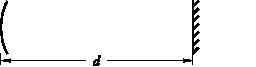
\includegraphics{figure/fig02.15a}
  } \\ \vspace{-0.3em}
  \subfigure[运动的雷达钟]{
    \label{fig:02.15b}
    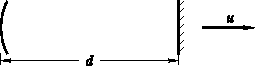
\includegraphics{figure/fig02.15b}
  } \\ \vspace{-0.3em}
  \subfigure[光信号向右传播]{
    \label{fig:02.15c}
    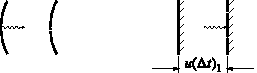
\includegraphics{figure/fig02.15c}
  } \\ \vspace{-0.3em}
  \subfigure[光信号向左传播]{
    \label{fig:02.15d}
    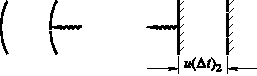
\includegraphics{figure/fig02.15d}
  }
  \caption{}
  \label{fig:02.15}
\end{figure}
现在我们来证明式\eqref{eqn:02.08.01}。我们仍使用一个雷达钟。如
图\ref{fig:02.15a}\\所示,当雷达钟与地面相对静止时,从地面参考系,即$K$
% 083.jpg
系来观察,它的天线与反射面之间的距离为$ d$;当雷达钟以速度$u$
运动时\lbr 图\ref{fig:02.15b}\rbr ,由$K$系测得的距离表示为$d'$。

我们考察光信号来回一次的运动。由于光在传播过程中雷达
在不断地运动,所以,由$K$看来,光传播的距离并不是$d'$。例如,
当光向右传播,从天线到达反射面时,若所用的时间为$\left(\Delta t\right)_1$,则
所走过的距离应为$ d ' + u \left( \Delta t \right) _ { 1 }$,其中$ u \left( \Delta t\right) _ { 1 } $一项表示在$\left(\Delta t\right)_1$时
间中钟向右运动的距离\lbr 图\ref{fig:02.15c}\rbr 。这样,我们有
\begin{equation*}
  \left( \Delta t \right) _ { 1 } = \frac { d ' + u \left(\Delta t\right)_1 } { c }
\end{equation*}
或者
\begin{equation}\label{eqn:02.08.02}
  \left( \Delta t \right) _ { 1 } = \frac { d ' } { c - u }
\end{equation}
类似地,光从反射面到天线的传播过程所用的时间$ \left(\Delta t\right)_2 $应是
\begin{equation}\label{eqn:02.08.03}
  \left( \Delta t \right) _ { 2 } = \frac { d ' } { c + u }
\end{equation}
由式\eqref{eqn:02.08.02}及式\eqref{eqn:02.08.03}可以得到光信号一个来回耗费的时间
\begin{equation}\label{eqn:02.08.04}
  \Delta t = \left( \Delta t \right) _ { 1 } + \left( \Delta t \right) _ { 2 } = \frac { 2 c d ' } { c ^ { 2 } - u ^ { 2 } }
\end{equation}
这是$K$系看到的结果。

在$K'$系,即雷达钟参考系来看,这个过程仍由下式描写
\begin{equation*}
  \left( \Delta t \right) ' = \frac { 2 d } { c }
\end{equation*}
因为在$K'$系观察,钟的长度是$d$。这样,式\eqref{eqn:02.08.04}可以改写为
\begin{equation*}
  \Delta t = \frac { 1 } { 1 - \dfrac { u ^ { 2 } } { c ^ { 2 } } } \left ( \frac { d ' } { d } \right) \left( \Delta t \right) '
\end{equation*}
再由上节推知的时间关系式\eqref{eqn:02.07.01},上式就成为
\begin{equation*}
  d ' = d \sqrt { 1 - \frac { u ^ { 2 } } { c ^ { 2 } } }
\end{equation*}
% 084.jpg
\clearpage
\noindent 这就是式\eqref{eqn:02.08.01}。

本节和上节的讨论用的都是雷达钟,因此,就存在一个共同
的问题,即运动钟的变慢和运动尺的变短是否普遍?或者,这些
推论是否只反映了雷达钟本身的性质,如果选择其他的钟有没有
这种性质?这些问题我们留待第十一章再来讨论。
